% Drawing 80/03-7 -- folder 80, batch 03, archive page 57 (PDF page 58).
% Transcription: dessin à l'encre : six droites, deux verticales, deux presque horizontales et deux obliques, les obliques passant par les coins opposés du petit carré central et se coupant en son centre ; les quatre triangles du carré et les quatre régions qui le bordent sont marqués $3$, les régions des coins $4$, celles du haut « id » ; à droite, cinq points isolés
% Kind: six lines: a square and its two diagonals. Method 2 (schematic redraw from the facsimile). Status: ok.
% Notes: Ink. Two verticals, two near-horizontals and two obliques; each oblique is drawn through two opposite corners of the central square (four triple points) and they cross at the computed centre. Labels 3 (eight), 4 (four) and « id » (four) as on the page: twelve regions. Five isolated dots at the right (the transcription's note counts four; the fifth is a blot with a short tail). Disagreement with the note: the centre is a square cut by its two diagonals, not a small triangle. Redrawn 2026-11-12 (issue 128): to check again.
% Coordinates: 1 unit = 1 mm = 1/100 of the crop width (bbox in page fractions: [0.2, 0.1, 0.95, 0.44]).
% Redrawn by Claude (claude-fable-5-2), issue #128, 2026-11-12; not checked by a human; not compiled (no TeX in the session).
% Rights: reproduces part of the work -- behind RENDER_TRANSCRIPTS, never published by itself.
\documentclass[tikz,border=3pt]{standalone}
\usepackage{amsmath,amssymb}
\usetikzlibrary{patterns,arrows.meta}
\tikzset{pencil/.style={black!45}, struck/.style={black!35}, mpt/.style={circle,draw,inner sep=1.3pt}, pt/.style={circle,fill,inner sep=0.9pt}, opt/.style={circle,draw,fill=white,inner sep=1.1pt}}
\begin{document}
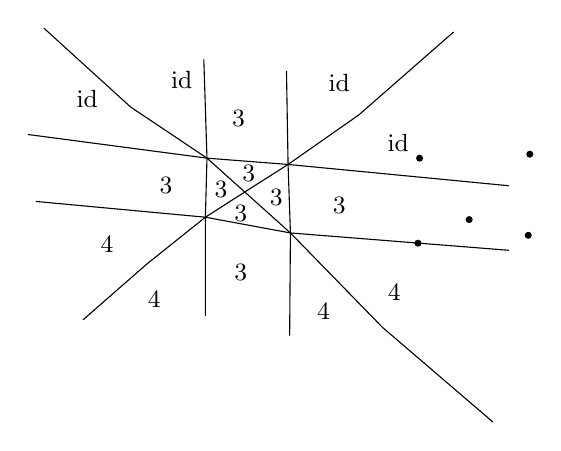
\begin{tikzpicture}[x=1mm,y=1mm,line cap=round,line join=round,font=\scriptsize]
\draw (26.3,-13) -- (26.7,-25.5) -- (26.5,-33) -- (26.5,-45.5);
\draw (36.8,-14.5) -- (37,-26.3) -- (37.3,-35) -- (37.2,-48);
\draw (4,-22.5) -- (26.7,-25.5) -- (37,-26.3) -- (65,-29);
\draw (5,-31) -- (26.5,-33) -- (37.3,-35) -- (65,-37.2);
\draw (6,-9) -- (17,-19) -- (26.7,-25.5) -- (31.5,-29.8) -- (37.3,-35) -- (49,-47) -- (63,-59);
\draw (58,-9.5) -- (46,-20) -- (37,-26.3) -- (31.5,-29.8) -- (26.5,-33) -- (19,-39) -- (11,-46);
\node[pt] at (53.7,-25.5) {};
\node[pt] at (67.7,-25) {};
\node[pt] at (53.5,-36.3) {};
\node[pt] at (67.5,-35.3) {};
\node[pt] at (60,-33.3) {};
\node[inner sep=1pt] at (28.5,-29.5) {\small $3$};
\node[inner sep=1pt] at (32,-27.5) {\small $3$};
\node[inner sep=1pt] at (35.5,-30.5) {\small $3$};
\node[inner sep=1pt] at (31,-32.5) {\small $3$};
\node[inner sep=1pt] at (30.7,-20.5) {\small $3$};
\node[inner sep=1pt] at (21.5,-29) {\small $3$};
\node[inner sep=1pt] at (43.5,-31.5) {\small $3$};
\node[inner sep=1pt] at (31,-40) {\small $3$};
\node[inner sep=1pt] at (14,-36.5) {\small $4$};
\node[inner sep=1pt] at (20,-43.5) {\small $4$};
\node[inner sep=1pt] at (41.5,-45) {\small $4$};
\node[inner sep=1pt] at (50.5,-42.5) {\small $4$};
\node[inner sep=1pt] at (11.5,-18) {\small id};
\node[inner sep=1pt] at (23.5,-15.5) {\small id};
\node[inner sep=1pt] at (43.5,-16) {\small id};
\node[inner sep=1pt] at (51,-23.5) {\small id};
\end{tikzpicture}
\end{document}
